
Gumbel statistics are often used to estimate the statistical
significance of local alignment scores.

The Gumbel distribution is the so-called Type I extreme value
distribution (EVD). It occurs so frequently in sequence analysis
applications, compared to the type II (Fr\'{e}chet) and type III
(Weibull) extreme value distributions, that ``Gumbel'' and ``EVD'' are
often used interchangeably in bioinformatics. Easel has a separate
module, the \eslmod{gev} module, that implements the generalized
extreme value distribution.

Karlin/Altschul statistics are a special case of the Gumbel
distribution that apply to the scores of ungapped local alignments
between infinitely long random sequences. Empirically, Karlin/Altschul
statistics also apply reasonably well to the more useful case of
gapped alignment of finite-length sequences. Karlin/Altschul
statistics predict how the Gumbel's two parameters depend on the
length of the query and target sequences. In the case of ungapped
alignments, Karlin/Altschul statistics allow the Gumbel parameters to
be estimated directly, without the need for a compute-intensive
simulation.

\subsection{The gumbel API}

The \eslmod{gumbel} API consists of the following functions:

\vspace{0.5em}
\begin{center}
\begin{tabular}{ll}\hline
    \multicolumn{2}{c}{\textbf{evaluating densities and distributions:}}\\
\ccode{esl\_gumbel\_pdf()}     & Returns the probability density, $P(S=x)$.\\
\ccode{esl\_gumbel\_logpdf()}  & Returns the log of the pdf, $\log P(S=x)$.\\
\ccode{esl\_gumbel\_cdf()}     & Returns the cumulative probability distribution, $P(S \leq x)$.\\
\ccode{esl\_gumbel\_logcdf()}  & Returns the log of the cdf, $\log P(S \leq x)$.\\
\ccode{esl\_gumbel\_surv()}    & Returns right tail mass, 1-cdf, $P(S > x)$\\
\ccode{esl\_gumbel\_logsurv()} & Returns log of 1-cdf, $\log P(S > x)$.\\
    \multicolumn{2}{c}{\textbf{sampling:}}\\
\ccode{esl\_gumbel\_Sample()}  & Returns a Gumbel-distributed random sample.\\
    \multicolumn{2}{c}{\textbf{maximum a posteriori parameter fitting:}}\\
\ccode{esl\_gumbel\_FitComplete()} & Estimates $\mu,\lambda$ from complete data.\\
\ccode{esl\_gumbel\_FitCompleteLoc()} & Estimates $\mu$ when $\lambda$ is known.\\
\ccode{esl\_gumbel\_FitCensored()} & Estimates $\mu,\lambda$ from censored data.\\
\ccode{esl\_gumbel\_FitCensoredLoc()} & Estimates $\mu$ when $\lambda$ is known.\\
\ccode{esl\_gumbel\_FitTruncated()}& Estimates $\mu,\lambda$ from truncated data.\\\hline
\end{tabular}
\end{center}
\vspace{0.5em}

The Gumbel distribution depends on two parameters, $\mu$ and
$\lambda$. When $\mu$ and $\lambda$ are known, the statistical
significance (P-value) of a single score $x$ is $P(S>x)$, obtained by
a call to \ccode{esl\_gumbel\_surv()}.  The E-value for obtaining that
score or better in searching a database of $N$ sequences is just
$NP(S>x)$.

When $\mu$ and $\lambda$ are unknown, they are estimated from scores
obtained from comparisons of simulated random data. (Analytical
solutions for $\mu$ and $\lambda$ are only available in the case of
ungapped sequence alignments.)  The \ccode{esl\_evd\_Fit*()} functions
provide maximum likelihood parameter fitting routines for different
types of data. 

\subsection{Example of using the gumbel API}

An example that samples 10,000 data points from a Gumbel distribution
with $\mu=-20$, $\lambda=0.4$; reports the min and max samples, and
the probability mass to the left of the min and to the right of the
max (both of which should be about $\frac{1}{10000}$, since we took
10,000 samples); and then fits those simulated data to a Gumbel and
reports the fitted $\mu$ and $\lambda$:

\input{cexcerpts/gumbel_example}



\subsection{Gumbel densities}

The probability density function (pdf) and the cumulative distribution
function (cdf) of the extreme value distribution are:

\begin{equation}
P(x) = \lambda \exp \left[ -\lambda (x - \mu) - e^{- \lambda (x - \mu)} \right]
\label{eqn:gumbel_density}
\end{equation}

\begin{equation}
P(S < x) = \exp \left[ -e^{-\lambda(x - \mu)} \right]
\label{eqn:gumbel_distribution}
\end{equation}

The extreme value density and distribution functions for $\mu = 0$ and
$\lambda = 1.0$ are shown below.

\begin{center}
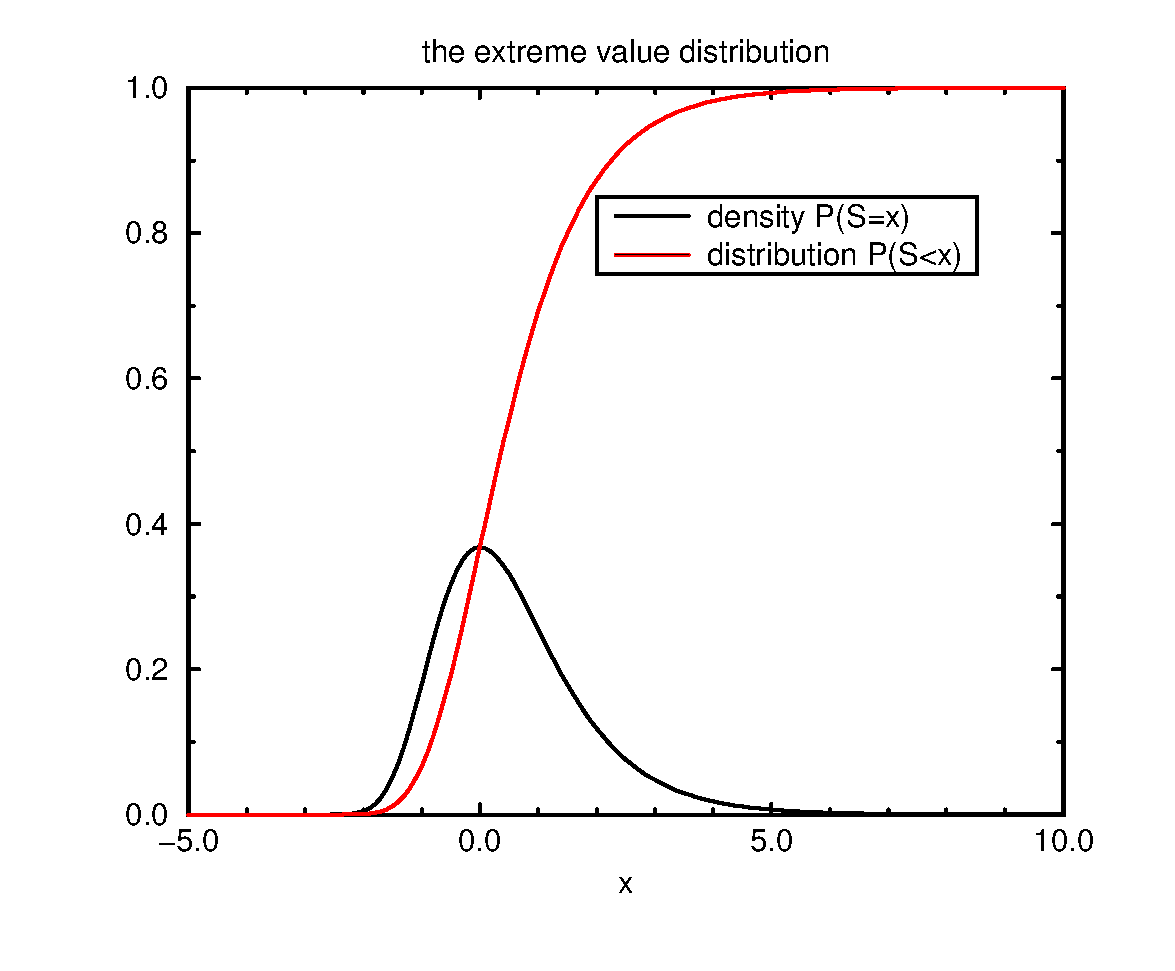
\includegraphics[width=3in]{figures/evd_basic}
\end{center}

The $\mu$ and $\lambda$ parameters are {\em location} and {\em scale}
parameters, respectively:

\centerline{
\begin{minipage}{3in}
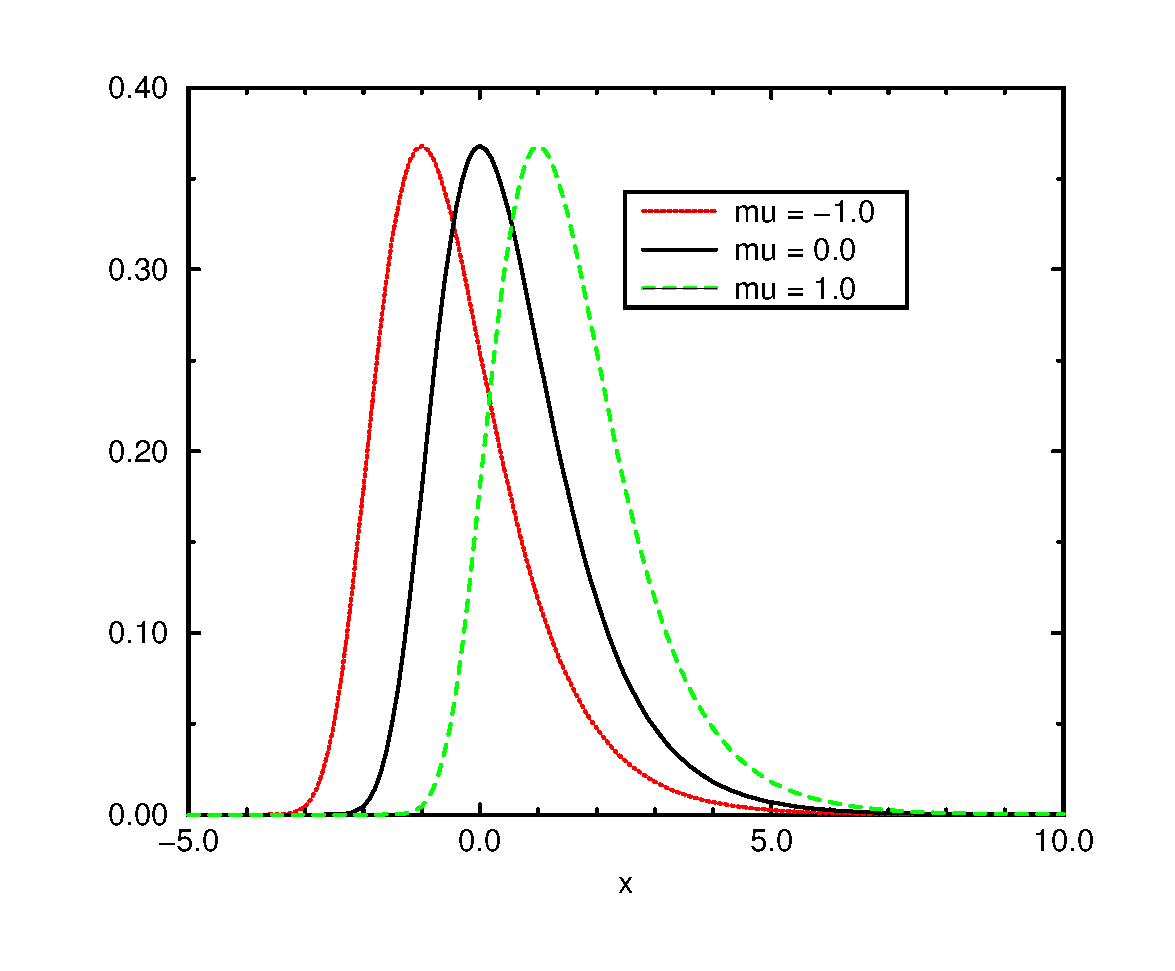
\includegraphics[width=2.8in]{figures/evd_location}
\end{minipage}
\begin{minipage}{3in}
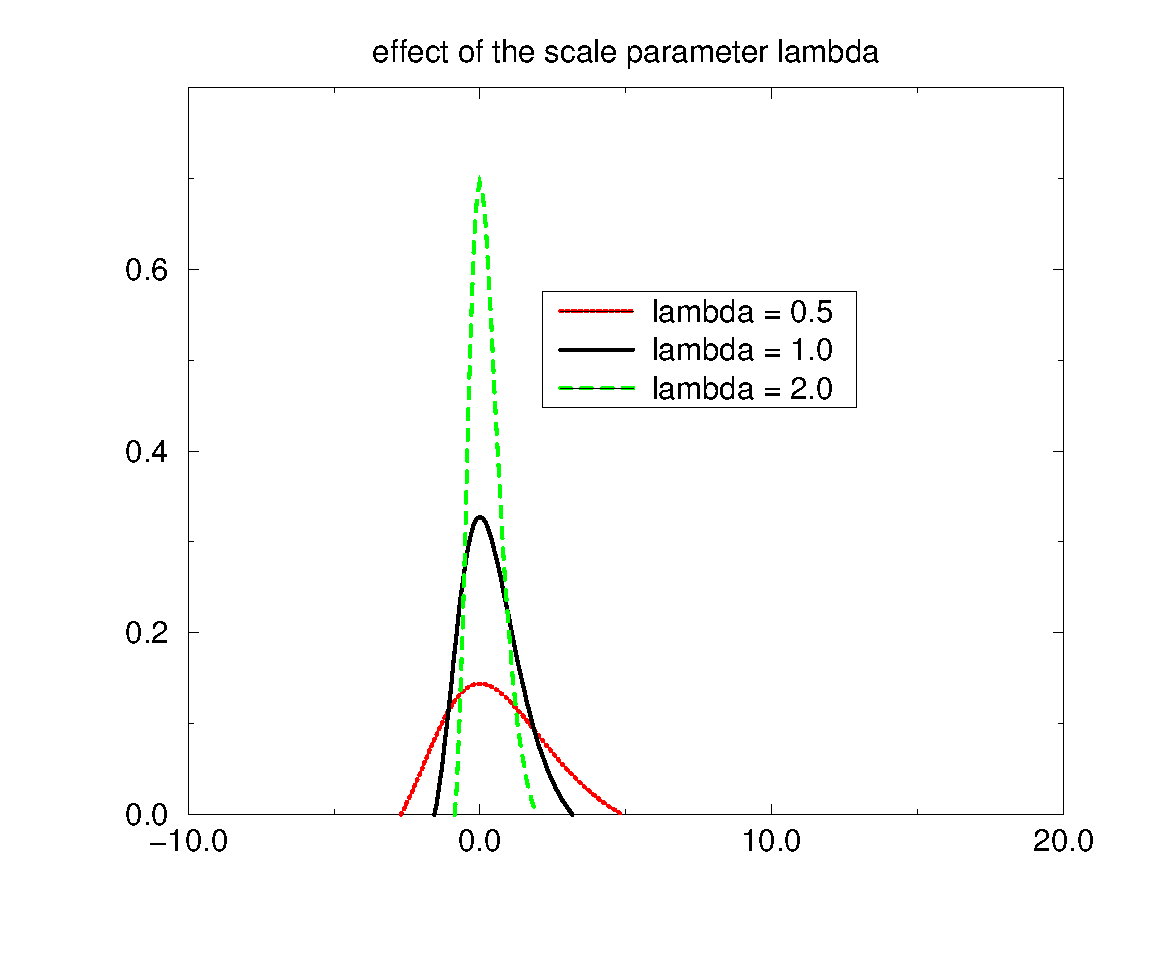
\includegraphics[width=2.8in]{figures/evd_scale}
\end{minipage}
}

For more details, a classic reference is \citep{Lawless82}.  Gumbel
distributions can have their long tail to the right or to the
left. The form given here is for the long tail to the right.  This is
the form that arises when the extreme value is a maximum, such as when
our score is the maximum over the individual scores of all possible
alignments. The equations in \citep{Lawless82} are for extremal
minima; use $(x - u) = -(x - \mu)$ and $b = 1 / \lambda$ to convert
Lawless' notation to the notation used here.


\subsection{Fitting Gumbel distributions to observed data}

Given a set of $n$ observed samples $\mathbf{x}$, we may want to
estimate the $\mu$ and $\lambda$ parameters.

One might try to use linear regression to fit to a $\log \log$
transformation of the $P(S < x)$ histogram, which gives a straight
line with slope $-\lambda$ and $x$ intercept $\mu$:

\begin{equation}
\log \left[ -\log P(S<x) \right] = -\lambda x + \lambda \mu
\end{equation}

However, the linear regression method is undesirable because it is
sensitive to outliers. The following table shows the \% error for
estimating $\hat{\mu}$ and $\hat{\lambda}$ from 500 simulated complete
datasets, sampled from a Gumbel with $\mu = -20.0$ and $\lambda =
0.4$, for four different dataset sizes:

\begin{center}
\begin{tabular}{lrrrr} \hline
                              & \multicolumn{4}{c}{\# of samples}\\
                              & 100 & 1000  & 10,000 & 100,000 \\
\% error in $\hat{\mu}$       &  2\%&   1\% & 0.9\%  &  0.9\%  \\
max error in $\hat{\mu}$      & 24\%&  13\% &  10\%  &   10\%  \\
\% error in $\hat{\lambda}$   & 12\%&   7\% &   5\%  &    3\%  \\
max error in $\hat{\lambda}$  & 49\%&  33\% &  25\%  &   20\%  \\ \hline
\end{tabular}
\end{center}


A better rough estimate of $\hat{\mu}$ and $\hat{\lambda}$ can be
obtained from the sample mean $m$ and variance $s^2$ of the observed
data \citep{Evans00}:\footnote{All simulation data are generated by
the \eslmod{evd} module's stats driver. The only exception is the
linear regression fit data, which come from an old version of HMMER.}

\begin{eqnarray*}
  \hat{\lambda} & = & \frac{\pi}{\sqrt{6s^2}}\\
  \hat{\mu}     & = & m - \frac{0.57722}{\hat{\lambda}}
\end{eqnarray*}

The mean/variance method is more accurate than linear regression, as
shown by the following simulation results:

\begin{center}
\begin{tabular}{lrrrr} \hline
                              & \multicolumn{4}{c}{\# of samples}\\
                              & 100 & 1000  & 10,000 & 100,000 \\
\% error in $\hat{\mu}$       &  1\%& 0.3\% &  0.1\% & 0.03\%  \\
max error in $\hat{\mu}$      &  5\%&   1\% &  0.4\% &  0.1\%  \\
\% error in $\hat{\lambda}$   &  9\%&   3\% &  0.8\% &  0.3\%  \\
max error in $\hat{\lambda}$  & 40\%&  12\% &    3\% &  0.9\%  \\ \hline
\end{tabular}
\end{center}

Still, the mean/variance method is not as accurate as a maximum
likelihood estimation (especially for $\lambda$). Also, it requires
complete data, whereas we also need to solve problems where we fit to
\emph{truncated} or \emph{censored} data. Easel's main estimation
methods are therefore maximum likelihood methods.

\subsubsection{Maximum likelihood estimation, complete data}

Given $n$ samples $x_1..x_n$ from some distribution that depends on
parameters $\theta$, we want to estimate maximum likelihood parameter
estimates $\hat{\theta}$ that maximize the log likelihood:

\[
   \hat{\theta} = \argmax_{\theta} \sum_{i=1}^{n} \log P(x_i \mid \theta)
\]

These are also \emph{maximum a posteriori} parameter estimates, if we
assume a uniform prior $P(\theta)$.

Specifically, for samples $x_i$ drawn from an extreme value
distribution, the log likelihood to optimize is:

\begin{equation}
\log L(\lambda, \mu) = n \log \lambda - \sum_{i=1}^{n} \lambda(x_i -
\mu) - \sum_{i=1}^{n} e^{-\lambda(x_i - \mu)}
\label{eqn:gumbel_logL}
\end{equation}

This objective function is differentiable with respect to $\mu$ and
$\lambda$:

\begin{eqnarray}
\frac{\partial \log L}{\partial \mu} & = &
n \lambda - \lambda \sum_{i=1}^{n} e^{-\lambda (x_i - \mu)}\\%
\\%
\label{eqn:mupartial}
\frac{\partial \log L}{\partial \lambda} & = &
\frac{n}{\lambda} - \sum_{i=1}^{n} (x_i - \mu) +  
\sum_{i=1}^{n} (x_i - \mu) e^{-\lambda (x_i - \mu)}
\label{eqn:lambdapartial}
\end{eqnarray}

The maximum likelihood estimates $\hat{\lambda}$ and $\hat{\mu}$ are
the solutions to $\frac{\partial \log L}{\partial \mu} = 0$ and
$\frac{\partial \log L}{\partial \lambda} = 0$. Lawless
\citep{Lawless82} gives a useful trick here that lets us solve both of
these simultaneously. When (\ref{eqn:mupartial}) is set to zero, it
can be used to get $\hat{\mu}$ in terms of $\hat{\lambda}$:

\begin{eqnarray}
e^{-\hat{\lambda} \hat{\mu}} & = & \frac{1}{n} \sum_{i=1}^{n} e^{-\hat{\lambda} x_i} 
\label{eqn:substitute}\\
\hat{\mu} & = & - \frac{1}{\hat{\lambda}} 
	\log \left[ \frac{1}{n} \sum_{i=1}^{n} e^{-\hat{\lambda} x_i} \right]
\label{eqn:solvemu}
\end{eqnarray}

Substituting (\ref{eqn:substitute}) into (\ref{eqn:lambdapartial}),
gives us an equation for solving $\hat{\lambda}$ in terms of the
$x_i$'s:

\begin{eqnarray}
\frac{1}{\hat{\lambda}} - \frac{1}{n} \sum_{i=1}^{n} x_i +
\frac{\sum_{i=1}^{n} x_i e^{-\hat{\lambda} x_i}}
     {\sum_{i=1}^{n} e^{-\hat{\lambda} x_i}} 
& = & 0
\label{eqn:newtontarget}
\end{eqnarray}

This is our target function. We could solve it readily enough (by
bisection search, for example) and obtain $\hat{\lambda}$. We can
solve it even faster using the Newton/Raphson algorithm, because it is
differentiable with respect to lambda:

\begin{equation}
\frac{d}{d\hat{\lambda}} = 
\frac{\left( \sum_{i=1}^{n} x_i e^{-\hat{\lambda} x_i} \right)^2 } 
     {\left( \sum_{i=1}^{n} e^{-\hat{\lambda} x_i}     \right)^2 }
-
\frac{\sum_{i=1}^{n} x_i^2 e^{-\hat{\lambda} x_i}}
     {\sum_{i=1}^{n} e^{-\hat{\lambda} x_i}}
-
\frac{1}{\hat{\lambda}^2}
\label{eqn:newtonderivative}
\end{equation}

Now, the key equations are (\ref{eqn:solvemu}),
(\ref{eqn:newtontarget}), and (\ref{eqn:newtonderivative}). In
summary, the inference procedure is the following:

\begin{itemize}
\item Guess an initial $\hat{\lambda}$ (using the mean/variance
  method, for example, but any reasonable guess works).
\item Use Newton/Raphson iterations to find the $\hat{\lambda}$ that satisfies
      (\ref{eqn:newtontarget}):
	\begin{itemize}
	\item calculate the target function $f$ and 
         its first derivative $f'$ at $\hat{\lambda}$, using 
	(\ref{eqn:newtontarget}) to calculate $f$ and 
	(\ref{eqn:newtonderivative}) to calculate $f'$.
	\item If $f$ is within some absolute tolerance of zero 
	(e.g., $10^{-6}$), stop; we have found $\hat{\lambda}$.
	\item Else, estimate a new $\hat{\lambda} = \hat{\lambda} - \frac{f}{f'}$,
	  and do another iteration.
	\end{itemize}
\item Plug $\hat{\lambda}$ into (\ref{eqn:solvemu}) to get $\hat{\mu}$.
\end{itemize}

This algorithm is implemented in \ccode{esl\_evd\_FitComplete()}.  An
auxiliary function, \ccode{lawless416()}, calculates the target
function and its derivative (equations (\ref{eqn:newtontarget}) and
(\ref{eqn:newtonderivative})) given the current estimate of
$\hat{\lambda}$.  The name comes from Lawless' equation 4.1.6, the
target function \citep{Lawless82}.

The accuracy of fitting to simulated data (generated with $\mu=-20$
and $\lambda=0.4$), collated over 500 simulations, is shown in the
following table:

\begin{center}
\begin{tabular}{lrrrr} \hline
                              & \multicolumn{4}{c}{\# of samples}\\
                              & 100 & 1000  & 10,000 & 100,000 \\
\% error in $\hat{\mu}$       &  1\%& 0.3\% &  0.1\% & 0.03\%  \\
max error in $\hat{\mu}$      &  4\%&   2\% &  0.5\% &  0.1\%  \\
\% error in $\hat{\lambda}$   &  6\%&   2\% &  0.6\% &  0.2\%  \\
max error in $\hat{\lambda}$  & 36\%&   9\% &    2\% &  0.8\%  \\ \hline
\end{tabular}
\end{center}

This is in accord with theoretical expectation. The distribution of
$\frac{\lambda}{\hat{\lambda}}$ is approximately normal with mean 1 and
standard error $\frac{0.78}{\sqrt{N}}$ \citep{Lawless82,Altschul01}. 

% Altschul says \frac{\hat{\lambda}}{\lambda}, actually, but I believe
% that's wrong. xref J1/46.


\subsubsection{Maximum likelihood fitting to censored data}

A \emph{censored} data problem is when we have $N$ samples, but we
only observe the values of a subset of $n$ samples $x_1..x_n$ that are
greater or equal to some cutoff $\phi$. The remaining $z = N-n$
samples are \emph{censored}, and for these we only know that $x <
\phi$.  $x_i..x_n$, $n$, $\phi$, and $z$ are all known in a censored
data problem.

To estimate maximum likelihood parameters $\hat{\theta}$ for some
distribution from censored data \citep{Gelman95}, the log likelihood
to maximize is:


\[ 
  \hat{\theta} = \argmax_{\theta} z \log P(x<\phi \mid \theta)
                         + \sum_{i=1}^n \log P(x_i \mid \theta)
\]

Specifically, when fitting a Gumbel distribution, the log likelihood
to optimize is:

\begin{equation}
  \log L(\lambda, \mu) = 
    n \log \lambda 
     - z e^{-\lambda(\phi - \mu)}
     - \sum_{i=1}^{n} \lambda(x_i - \mu) 
     - \sum_{i=1}^{n} e^{-\lambda(x_i - \mu)}
\label{eqn:censor_logL}
\end{equation}

To optimize this, we follow a similar procedure as used for complete
data \citep{Lawless82}. The log likelihood is differentiable with
respect to $\lambda$ and $\mu$:

\begin{eqnarray}
\frac{\partial \log L}{\partial \mu} & = &
n \lambda  
- z \lambda e^{-\lambda (\phi - \mu)}
- \lambda \sum_{i=1}^{n} e^{-\lambda (x_i - \mu)}
\label{eqn:censor_dmu}
\\%
\frac{\partial \log L}{\partial \lambda} & = &
\frac{n}{\lambda} 
+ z (\phi - \mu) e^{-\lambda (\phi - \mu)}
- \sum_{i=1}^{n} (x_i - \mu) 
+ \sum_{i=1}^{n} (x_i - \mu) e^{-\lambda (x_i - \mu)}
\label{eqn:censor_dlambda}
\end{eqnarray}

Setting (\ref{eqn:censor_dmu}) to zero and solving for $\hat{\mu}$ in
terms of $\hat{\lambda}$ gives:

\begin{equation}
\hat{\mu}  =  - \frac{1}{\hat{\lambda}} 
	\log \left[ \frac{1}{n} 
	\left( z e^{-\hat{\lambda} \phi} 
               + \sum_{i=1}^{n} e^{-\hat{\lambda} x_i} \right)
	\right]
\label{eqn:censor_solvemu}
\end{equation}

Substituting (\ref{eqn:censor_solvemu}) into
(\ref{eqn:censor_dlambda}) gives the target equation:

\begin{equation}
\frac{1}{\hat{\lambda}} 
- \frac{1}{n} \sum_{i=1}^{n} x_i +
\frac{z \phi e^{-\hat{\lambda} \phi} + \sum_{i=1}^{n} x_i e^{-\hat{\lambda} x_i}} 
     {z e^{-\hat{\lambda} \phi} + \sum_{i=1}^{n} e^{-\hat{\lambda} x_i}} 
 =  0
\label{eqn:censor_newtontarget}
\end{equation}

To use Newton-Raphson root finding (instead of a slower bisection
search) we also need the first derivative of this target equation with
respect to $\lambda$:

\begin{equation}
\frac{d}{d\hat{\lambda}} = 
\frac{\left( 
        z \phi e^{-\hat{\lambda} \phi}
        + \sum_{i=1}^{n} x_i e^{-\hat{\lambda} x_i} 
       \right)^2 } 
     {\left( 
        z e^{-\hat{\lambda} \phi}
        + \sum_{i=1}^{n} e^{-\hat{\lambda} x_i}     
       \right)^2 }
-
\frac{z \phi^2 e^{-\hat{\lambda} \phi} + \sum_{i=1}^{n} x_i^2 e^{-\hat{\lambda} x_i}}
     {z  e^{-\hat{\lambda} \phi} + \sum_{i=1}^{n} e^{-\hat{\lambda} x_i}}
-
\frac{1}{\hat{\lambda}^2}
\label{eqn:censor_newtonderiv}
\end{equation}

In summary: given $n$ observed samples $x_1..x_n$ from a total sample
of $N$ samples, $z = N-n$ of which were censored because they have
values $< \phi$, we solve for maximum likelihood estimates
$\hat{\lambda}$ and $\hat{\mu}$ using the same procedure we used for
complete data, by using equations (\ref{eqn:censor_solvemu}),
(\ref{eqn:censor_newtontarget}), and (\ref{eqn:censor_newtonderiv}) in
place of equations (\ref{eqn:solvemu}), (\ref{eqn:newtontarget}), and
(\ref{eqn:newtonderivative}). Easel implements this procedure in
\ccode{esl\_evd\_FitCensored()}.  The target function
(\ref{eqn:censor_newtontarget}) and its derivative
(\ref{eqn:censor_newtonderiv}) are implemented in the auxiliary
function \ccode{lawless422()} \citep{Lawless82}.

Results on 500 simulated datasets with $\mu = -20, \lambda = 0.4$,
censored at $\phi = -20$ -- the expected peak of the histogram; that
is, a censored fit only to the right tail, which contains about 63\%
of the samples:

\begin{center}
\begin{tabular}{lrrrr} \hline
 & \multicolumn{4}{c}{\# samples in EVD histogram}\\
                        & 100 & 1000  & 10,000 & 100,000 \\
\% error in $\mu$       &  1\%& 0.4\% &  0.1\% &  0.04\%  \\
max error in $\mu$      &  5\%&   2\% &  0.5\% &  0.2\%  \\
\% error in $\lambda$   &  9\%&   3\% &  0.9\% &  0.3\%  \\
max error in $\lambda$  & 33\%&  11\% &    3\% &    1\%  \\ \hline
\end{tabular}
\end{center}

\subsubsection{Maximum likelihood fitting to truncated data}

A \emph{truncated} dataset is when we only observe $n$ samples $x_i$,
and an \emph{unknown} number $z$ of samples less than some threshold
$\phi$ were unobserved. Thus, only the right tail of $n$ samples $x_i
\geq \phi$ as observed. In a truncated dataset, $x_1..x_n$, $n$, and
$\phi$ are known, but $z$ is unknown.

Solving a truncated data problem motivates a Bayesian approach,
because we need to integrate out (marginalize) the nuisance $z$
parameter, and to do this, we have to specify a prior distribution for
$P(z)$. Gelman \emph{et al.} describe a general Bayesian framework for
thinking about various types of missing data problems, including
censored and truncated data \citep{Gelman95}.

In short, to obtain maximum likelihood parameters $\hat{\theta}$ for
some distribution, given truncated data, the log likelihood we wish to
maximize is:

\begin{equation}
  \hat{\theta} = \argmax_\theta -n \log P(x \geq \phi \mid \theta) 
                   + \sum_{i=1}^n \log P(x_i \mid \theta).
\label{eqn:truncated_objective}
\end{equation}

\textbf{Detour: derivation of the truncated data likelihood}

The derivation of the above equation may not be immediately obvious.
The presence of the $n P(x \geq \phi \mid \theta)$ term may be
counterintuitive, as opposed to the more intuitive $z P(x < \phi \mid
\theta)$ term that accounts for the missing data in a censored data
problem. Gelman \emph{et al.} actually don't even show the equation in
their book; I obtained it from an exercise solution on their web site.
To convince you (and to remind me) of its correctness, a sketch of the
derivation follows.

We start with the same likelihood equation that arises in censored
data for a \emph{known} total number of samples $N$ (where $N=n+z$),
but since $N$ is unknown, we need to integrate over all possible $N$
from $n$ to $\infty$:

\begin{eqnarray*}
   P(\mathbf{x} \mid \theta, \phi) & = &
    \sum_{N=n}^{\infty}   P(\mathbf{x} \mid \theta, \phi, N) P(N)\\
   & = & 
    \prod_{i=1}^n P(x_i \mid \theta) 
    \left[
      \sum_{N=n}^\infty {N \choose n} P(x < \phi \mid \theta)^{N-n} P(N)
    \right]\\
\end{eqnarray*}

The $\prod_{i=1}^n P(x_i \mid \theta)$ is straightforward; that sum is
our problem. The trick is to rearrange it so we can treat it as a
convergent negative binomial series:

\[
   (1-p)^{-a} = 1 + ap + \frac{a(a+1)}{2!} p^2 +
   \frac{a(a+1)(a+2)}{3!} p^3...
\]

To get the sum into the form of this series, Gelman \emph{et al.}
suggest using an informative prior $P(N) = \frac{1}{N}$, an apparently
unmotivated choice that happens to make the sum collapse nicely:

\begin{eqnarray*}
 &=& P(N=n) 
    + (n+1) P(x < \phi \mid \theta) P(N=n+1) 
    + \frac{(n+1)(n+2)}{2!} P(x < \phi \mid \theta)^2 P(N=n+2) ...\\
 &= & \frac{1}{n} \left[
      1 
      + n P(x < \phi \mid \theta)
      + \frac{n(n+1)}{2!} P(x < \phi \mid \theta)^2 
      + \frac{n(n+1)(n+2)}{3!} P(x < \phi \mid \theta)^3 \right]\\
 &=& \frac{1}{n} (1 - P(x < \phi \mid \theta))^{-n}\\
 &=& \frac{1}{n} P(x \geq \phi \mid \theta)^{-n}\\
\end{eqnarray*}

The $\frac{1}{n}$ is a constant, so we drop it from the likelihood
equation we'll maximize. Putting this term back together with the
probability of the observed data and taking the log, we obtain the log
likelihood in equation (\ref{eqn:truncated_objective}).

Alternatively, we might choose an uninformative improper uniform prior
$P(N) \propto 1$. This gives a log likelihood that only differs by a
term of $n+1$ versus $n$:

\begin{equation}
  \hat{\theta} = \argmax_\theta -(n+1) \log P(x \geq \phi \mid \theta) 
                   + \sum_{i=1}^n \log P(x_i \mid \theta).
\end{equation}

However, empirically, this form is ineffective, at least for fitting
Gumbels. The $\frac{1}{N}$ prior performs much better, probably
because it constrains the solutions to favor smaller, finite, more
reasonable choices of $N$.



\textbf{Back to fitting a truncated Gumbel}

For the specific case of fitting a truncated Gumbel, the log
likelihood (\ref{eqn:truncated_objective}) to optimize is:

\[
  \log L(\lambda, \mu) =
     n \log \lambda 
     - \sum_{i=1}^{n} \lambda(x_i - \mu) 
     - \sum_{i=1}^{n} e^{-\lambda(x_i - \mu)}
     - n \log (1 - \exp(-e^{-\lambda(\phi - \mu)}))
\label{eqn:truncated_logL}
\]

This is differentiable with respect to $\lambda$ and $\mu$, but it's
not going to reduce to the clean root-finding problem that we obtained
for complete data or censored data. Instead we're going to be left
with a numerical optimization problem. We can use standard numerical
optimization code, such as steepest descent or conjugate gradient
descent. There's just one hitch. These algorithms assume unconstrained
parameters, but $\lambda$ is constrained to values $>0$. We do a
change of variables, and use the transformation $\lambda = e^w$ so we
can optimize the unconstrained parameter $w = \log \lambda$ instead of
optimizing $\lambda$ directly.  The necessary partial derivatives are
then:

\begin{eqnarray}
\frac{\partial \log L}{\partial \mu} & = &
n \lambda  
- \lambda \sum_{i=1}^{n} e^{-\lambda (x_i - \mu)}
- \frac{n \lambda \exp \left[ -\lambda (\phi - \mu) - e^{- \lambda (\phi - \mu)} \right]}
       {1 - \exp(-e^{-\lambda(\phi - \mu)})}
\label{eqn:truncated_dmu}
\\%
\frac{\partial \log L}{\partial w} & = &
n 
- \sum_{i=1}^{n} \lambda(x_i - \mu) 
+ \sum_{i=1}^{n} \lambda(x_i - \mu) e^{-\lambda (x_i - \mu)}
+ \frac{n\lambda (\phi-\mu) \exp \left[ -\lambda (\phi - \mu) - e^{- \lambda (\phi - \mu)} \right]}
       {1 - \exp(-e^{-\lambda(\phi - \mu)})}
\label{eqn:truncated_dw}
\end{eqnarray}

This optimization is carried out by \ccode{esl\_evd\_FitTruncated()}.
The likelihood (\ref{eqn:truncated_logL}) is implemented in
\ccode{tevd\_func()}, and the derivatives (\ref{eqn:truncated_dmu}) and
(\ref{eqn:truncated_dw}) are implemented in \ccode{tevd\_dfunc()}.
\ccode{esl\_evd\_FitTruncated()} simply sets up the problem and passes
it all off to a conjugate gradient descent optimizer.

Results on 500 simulated datasets with $\mu = -20, \lambda = 0.4$,
truncated at $\phi = -20$ (leaving the right tail, containing about
63\% of the samples):

\begin{center}
\begin{tabular}{lrrrr} \hline
                              & \multicolumn{4}{c}{\# samples}\\
                              & 100 & 1000  & 10,000 & 100,000 \\
\% error in $\hat{\mu}$       & 13\%&   2\% &  0.8\% &  0.3\%  \\
max error in $\hat{\mu}$      &260\%&  42\% &    3\% &    1\%  \\
\% error in $\hat{\lambda}$   & 15\%&   5\% &    2\% &  0.6\%  \\
max error in $\hat{\lambda}$  & 68\%&  18\% &    6\% &    2\%  \\ \hline
\end{tabular}
\end{center}

Fitting truncated Gumbel distributions is difficult, requiring much
more data than fitting complete or censored data. The problem is that
the right tail becomes a scale-free exponential when $\phi >> \mu$,
and $\mu$ becomes undetermined. Fits become very inaccurate as $\phi$
gets larger than $\mu$, and for sufficiently large $\phi$, the
numerical optimizer will completely fail.







